\documentclass[expologarit]{subfiles}
\begin{document}

 \begin{center}
\color{violet} \kml លំហាត់ទី១០
 \end{center}
គេមានអនុគមន៍ $f$ កំណត់ដោយ $f(x)=\frac{2x^2-7x+5}{x^2-5x+7}$ ។\\ យើងតាងដោយ $(C)$ ក្រាបរបស់វាលើតម្រុយអរតូណរម៉ាល់ $\left(O,\overrightarrow{i},\overrightarrow{j}\right)$ ។
\begin{enumerate}
\item រកដែនកំណត់ $D$ នៃអនុគមន៍ $f$ ។
\item សិក្សាលីមីតនៃអនុគមន៍ $f(x)$ ត្រង់ $-\infty$ និងត្រង់ $+\infty$។\\ ទាញរកសមីការអាស៊ីមតូត $d$ ទៅនឹងក្រាប$(C)$ ត្រង់ $-\infty$ និងត្រង់ $+\infty$។
\item \begin{enumerate}[a]
\item ស្រាយបំភ្លឺថាគ្រប់ចំនួនពិត $x\in D;\ $ ដេរីវេ $f'(x)=\frac{-3\left(x^2-6x+8\right)}{\left(x^2-5x+7\right)^2}$ ។
\item សិក្សាអថេរភាពនៃអនុគមន៍ $f$ និងសង់តារាងអថេរភាពនៃអនុគមន៍ $f$។
\item សង់ក្រាប$(C)$ នៃអនុគមន៍$f $។
\end{enumerate}
\end{enumerate}
\begin{center}
\color{violet}\kml ដំណោះស្រាយ
\end{center}
\begin{enumerate}
\item រកដែនកំណត់ $D$ នៃអនុគមន៍ $f$ 
\\[0.25cm]
យើងមាន $f(x)=\frac{2x^2-7x+5}{x^2-5x+7}$ \\[0.25cm]
$f(x)$ មានន័យលុះត្រាតែ $x^2-5x+7\neq 0$ 
\begin{flalign*}
& \Delta =b^2-4ac=(-5)^2-4(1)(7)=25-28=-3<0\quad & \\ 
& \Rightarrow \ x^2-5x+7 \ \text{មានសញ្ញាដូចមេគុណ$a$} 
\end{flalign*}
យើងបាន $x^2-5x+7>0\quad \forall\ x\in\mathbb{R}$\\[0.25cm]
ដូចនេះ \fbox{$D_f=\mathbb{R}$}
\item សិក្សាលីមីតនៃអនុគមន៍ $f(x)$ ត្រង់ $-\infty$ និងត្រង់ $+\infty$
\begin{flalign*}
&\lim_{x\to -\infty}f(x)=\lim_{x\to -\infty}\frac{2x^2-7x+5}{x^2-5x+7}=\lim_{x\to -\infty}\frac{x^2\left(2-\frac{7}{x}+\frac{5}{x^2}\right)}{x^2\left(1-\frac{5}{x}+\frac{7}{x^2}\right)}=2&\\
&\lim_{x\to +\infty}f(x)=\lim_{x\to +\infty}\frac{2x^2-7x+5}{x^2-5x+7}=\lim_{x\to +\infty}\frac{x^2\left(2-\frac{7}{x}+\frac{5}{x^2}\right)}{x^2\left(1-\frac{5}{x}+\frac{7}{x^2}\right)}=2
\end{flalign*}
 ទាញរកសមីការអាស៊ីមតូត $d$ ទៅនឹងក្រាប$(C)$ ត្រង់ $-\infty$ និងត្រង់ $+\infty$
 \\
 ដោយ $\lim_{x\to \pm\infty}f(x)=2$\quad  ដូចនេះ \fbox{បន្ទាត់ $y=2$ ជាអាស៊ីមតូតដេកនៃក្រាប$(C)$}
\item \begin{enumerate}[a]
\item ស្រាយបំភ្លឺថាគ្រប់ចំនួនពិត $x\in D;\ $ ដេរីវេ $f'(x)=\frac{-3\left(x^2-6x+8\right)}{\left(x^2-5x+7\right)^2}$ 
\begin{flalign*}
f'(x)=\left(\frac{2x^2-7x+5}{x^2-5x+7}\right)'&=\frac{(4x-7)\left(x^2-5x+7\right)-(2x-5)\left(2x^2-7x+5\right)}{\left(x^2-5x+7\right)^2}&\\
&=\frac{-3x^2+18x-24}{\left(x^2-5x+7\right)^2}\\
&=\frac{-3\left(x^2-6x+8\right)}{\left(x^2-5x+7\right)^2}
\end{flalign*}
ដូចនេះ \fbox{$x\in D;\ $ ដេរីវេ $f'(x)=\frac{-3\left(x^2-6x+8\right)}{\left(x^2-5x+7\right)^2}$}
\item សិក្សាអថេរភាពនៃអនុគមន៍ $f$ 
\begin{flalign*}
f'(x)=0\Leftrightarrow\quad & -3\left(x^2-6x+8\right)=0  &\\
\Leftrightarrow\quad & -3x^2+18x-24=0 \\
\Leftrightarrow\quad & (-3x+6)(x-4)=0 \\
\Rightarrow\quad &\left[\begin{array}{l}
-3x+6=0\\
x-4=0
\end{array}\right. \quad \Rightarrow\left[\begin{array}{l}
x=2\\
x=4
\end{array}\right.
\end{flalign*}
 តារាសញ្ញាដេរីវេ $f'(x)$
\\[0.2cm]
\begin{tikzpicture}
   \tkzTabInit[lw=1,lgt=1.5,espcl=2]{$x$ / 0.75 , $f'(x)$ / 1}{$ -\infty$ , $2$,$4$, $+\infty $}
   \tkzTabLine{, -, z,+,z,-  }
\end{tikzpicture}
\newpage 
\begin{itemize}
\item $f'(x)>0$ ពេល $x\in\left(2,4\right)\quad\Rightarrow $\quad អនុគមន៍$f$ កើនលើចន្លោះ$x\in (2,4)$
\item $f'(x)<0$ ពេល $x\in\left(-\infty ,2\right)\cup \left(4,+\infty\right)$\\
$\Rightarrow $ អនុគមន៍$f$ ចុះលើចន្លោះ$x\in\left(-\infty ,2\right)\cup \left(4,+\infty\right)$
\end{itemize}
បរមាធៀប
\begin{itemize}
\item  ត្រង់ $x=2;\ f'(x)=0$ ហើយប្តូរសញ្ញាពី$-$ ទៅ$+$ យើងបាន $f$ មានអប្បបរមាធៀបមួយគឺ
\begin{flalign*}
f(2)=\frac{2(2)^2-7(2)+5}{(2)^2-5(2)+7}=-1&&
\end{flalign*}
\item ត្រង់ $x=4;\ f'(x)=0$ ហើយប្តូរសញ្ញាពី$+$ ទៅ$-$ យើងបាន $f$ មានអតិបរមាធៀបមួយគឺ
\begin{flalign*}
f(4)=\frac{2(4)^2-7(4)+5}{(4)^2-5(4)+7}=3 &&
\end{flalign*}
\end{itemize}
តារាងអថេរភាពនៃអនុគមន៍ $f$
\\[0.2cm]
\begin{tikzpicture}
   \tkzTabInit[lw=1,lgt=1.5,espcl=2]{$x$ / 0.75 , $f'(x)$ / 1,$f(x)$/2}{$ -\infty$ , $2$,$4$, $+\infty $}
   \tkzTabLine{, -, z,+,z,-  }
       \tkzTabVar{+/ $2$,-/$-1$ ,+/$3$, -/ $2$}
\end{tikzpicture}
\item សង់ក្រាប$(C)$ នៃអនុគមន៍$f $
\begin{flalign*}
(C)\cap (x'ox)\Leftrightarrow y=0\quad\Leftrightarrow\quad & 2x^2-7x+5=0&\\
 & \text{មានរាង}\ a+b+c=0\\
 \Rightarrow\quad & x_1=1,\ x_2=\frac{c}{a}=\frac{5}{2} 
\end{flalign*}
\vspace{-1cm}
\begin{flalign*}
&(C)\cap (y'oy)\Leftrightarrow x=0\quad\Rightarrow\quad y=\frac{2(0)^2-7(0)+5}{(0)^2-5(0)+7}=\frac{5}{7}&\\
&(C)\cap (d):y=2\Leftrightarrow  2=\frac{2x^2-7x+5}{x^2-5x+7} \quad\Rightarrow \quad x=3
\end{flalign*}
\end{enumerate}
\end{enumerate}
 \begin{center}
\begin{tikzpicture}[x=1cm,y=1cm]
\begin{axis}[scale=1,
          xmax=7.5,ymax=6.5,
          axis lines=middle,
          xmin=-5,ymin=-6.5,          
          xtick={-12,-11,...,10},
          ytick={-12,-11,...,12}  ,
          xlabel=$x$   ,
          ylabel=$y$   ,x=1cm, y=1cm
          ] 
\addplot[domain=-13:10 ,restrict y to domain=-14:14,line width=1pt,samples=1000,smooth,name path=A,color=red] {(2*x^2-7*x+5)/(x^2-5*x+7)};
\addplot[domain=-14.5:10,line width=1.5pt,samples=100,smooth,line width=1.5pt] {2}node[sloped, near end,above]{$\qquad\qquad\qquad\qquad\qquad
y=2$};

%\addplot [color=black]coordinates {(-2.5,0)} node[below ]{$x'$};

%\node at(0,-1){$\bullet$};

%\draw[dashed](1,0)--(1,1)--(0,1);

             %\addplot[gray, pattern=north west lines] fill between[of=A and B, soft clip={domain=1:2}];
            

       
        
  
              \draw (0,0)rectangle (0.2,0.2);
           
            \draw (-4.5,1) node {$(C)$};
             \draw [dashed](2,0)--(2,-1) node {$\bullet$}--(0,-1);
              \draw (1,0) node {$\bullet$};
                 \draw (2.5,0) node {$\bullet$};
                    \draw (0,0.7) node {$\bullet$};
                    
               \draw[dashed](4,0)-- (4,3) node {$\bullet$}--(0,3);
\end{axis}
\end{tikzpicture}
 \end{center}
\end{document}